\section{Distribuição amostral e $\chi^2$}
\begin{frame}{Distribuição amostral e $\chi^2$}
 \begin{itemize}
  \item Distribuição amostral de uma estatística;
  \item A família qui-quadrado de distribuições Gamma;
  \item Exemplos.
 \end{itemize}
\end{frame}
\begin{frame}{Distribuição amostral de uma estatística}
 Se $\bX = \{ \rs \}$ é uma amostra aleatória, $T = r(\rs)$ é uma variável aleatória, e portanto, faz sentido falar da distribuição de $T$.
 \begin{exemplo}[Distribuição amostral de uma proporção]
  (Exemplo 8.1.1 em De Groot)
  
  Suponha que estamos interessados na proporção de pacientes que se recrudescem após tratamento com uma determinada droga.
  Para uma amostra de $n$ pacientes, podemos modelar os desfechos como variáveis aleatórias i.i.d. Bernoulli com parâmetro $\theta$ e computar $T = n^{-1}\sum_{i=1}^n X_i$ como estimativa de $\theta$.
  Deste modo, temos
  \begin{equation}
  \label{eq:sampling_distribution_binomial}
   \pr(T = t) =
    \begin{cases}
    \binom{n}{nt} \theta^{nt} (1-\theta)^{n(1-t)}, t = \frac{0}{n}, \frac{1}{n}, \ldots,\frac{n-1}{n} ,\frac{n}{n},\\
    0,\text{caso contrário}.
    \end{cases}
  \end{equation}
Chamamos~(\ref{eq:sampling_distribution_binomial}) de~\textbf{distribuição amostral} de $T$.
 \end{exemplo}
\end{frame}

\begin{frame}{Fazendo afirmações probabilísticas sobre estimadores}
 Relembre o exemplo das lâmpadas de Astolfo:
 \[ \hat{\theta}_{\text{Bayes}} = \frac{\alpha + n}{\beta + S}; \: \hat{\theta}_{\text{EMV}} = \frac{n}{S}. \]
 Podemos perguntar, 
 \[ \pr\left(|\hat{\theta} -\theta| < a\right) = ? \]
\end{frame}

\begin{frame}{Ilustrando}
 \begin{figure}
  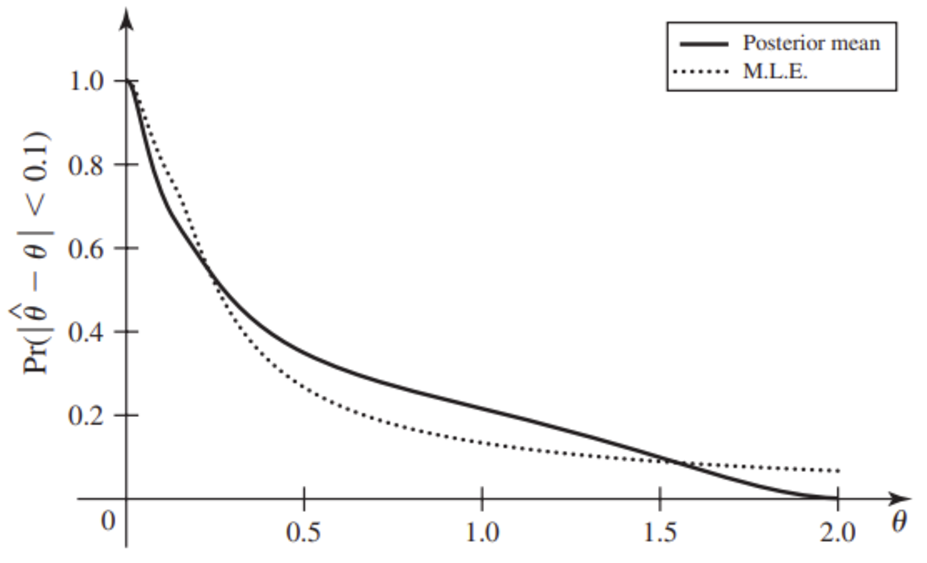
\includegraphics[scale=0.6]{figures/probability_curves_DeGroot8.1.pdf}
 \end{figure}
\end{frame}

\section{Qui-quadrado}

\begin{frame}{A distribuição qui-quadrado}
 \begin{defn}[Distribuição qui-quadrado]
 Dizemos que uma variável aleatória $Y$ tem distribuição~\textbf{qui-quadrado} com $m$ graus de liberdade quando
 \begin{equation}
 f_Y(y) = \frac{1}{2^{m/2}\Gamma(m/2)} y^{m/2 - 1}e^{-y/2}, \: y >0.
 \end{equation} 
 
 Vemos que $Y$ tem função geradora de momentos
\[\psi(t) = \left( \frac{1}{1-2t}\right)^{m/2}, t < 1/2 .\]
 \end{defn}
$E[Y] = ?$, $\vr(Y) =?$  
\end{frame}

\begin{frame}{Alguns resultados úteis}

\begin{theo}[Soma de variáveis aleatórias qui-quadrado]
Se $\rs$ são variáveis aleatórias independentes com graus de liberdade $m_i$, então $W = \sum_{i=1}^n X_i$ tem distribuição qui-quadrado com graus de liberdade $m =  \sum_{i=1}^n m_i$.
\end{theo}
\textbf{Prova}: Segue da soma de variáveis aleatórias Gama.

\begin{theo}[Distribuição do quadrado de uma variável aleatória Normal padrão]
Se $X \sim\operatorname{Normal}(0, 1)$, $Y = X^2$ tem distribuição qui-quadrado com $m=1$. 
\end{theo}
\textbf{Prova}: Escrever a acumulada de $Y$, diferenciar e usar a regra da cadeia.

\begin{obs}[Distribuição da soma de quadrados de normais padrão]
\label{rmk:sum_squares_standard_normal}
 Se $\rs$ são variáveis aleatórias Normal padrão, então $Z = \sum_{i=1}^n X_i^2$ tem distribuição qui-quadrado com $n$ graus de liberdade.
\end{obs}
\textbf{Prova}: Imediato dos dois últimos teoremas.

\end{frame}

\begin{frame}{Distribuição da variância amostral}
 Vamos a um exemplo motivador.
No caso Normal, quando $\mu$ é conhecida, temos o estimador de máxima verossimilhança para a variância:
\[ \hat{\sigma^2} = \frac{1}{n} \sum_{i=1}^n (X_i - \mu)^2. \]
Isso nos leva às duas próximas observações
\begin{obs}[Uma transformação linear do EMV]
 \begin{equation*}
  \frac{n\hat{\sigma^2}}{\sigma^2} \sim \operatorname{qui-quadrado}(n).
 \end{equation*}
\end{obs}
\textbf{Prova}: Notar que $Z_i = (X_i-\mu)/\sigma$ são Normal padrão e aplicar a observação~\ref{rmk:sum_squares_standard_normal}.

\begin{obs}[Distribuição do EMV da variância]
\label{rmk:sampling_distribution_normal_variance}
 \begin{equation*}
  \hat{\sigma^2} \sim \operatorname{Gama}\left(\frac{n}{2}, \frac{n}{2\sigma^2} \right).
 \end{equation*}

\end{obs}
\textbf{Prova}: Exercício 13 da seção 8.2 de DeGroot. 
\end{frame}

\begin{frame}{Quem comeu o meu queijo?}
 \begin{exemplo}[Concentração de ácido no queijo]
  Suponha que estamos interessados em medir a concentração de um certo ácido em pedaços de queijo produzidos por uma fábrica.
  Ao longo dos anos, grande acúmulo de dados permitiu afirmar que a distribuição populacional da concentração é Normal com parâmetros $\mu$ e $\sigma^2$.
  Suponha que amostramos $n$ pedaços e medimos as concentrações $\rs$.
  Então 
  \[ Y = \frac{1}{n}\sum_{i=1}^n |X_i-\mu|^2 \]
é uma medida de quanto estas amostras desviam da concentração típica $\mu$.
Suponha que uma diferença de concentração $u$ é o suficiente para dar gosto diferente ao queijo.
Podemos calcular $\pr(Y \leq u^2)$ para quantificar o risco de isso acontecer.
 \end{exemplo}

\end{frame}



\begin{frame}{O que aprendemos?}
\begin{itemize}

  \item[\faLightbulbO] Distribuição amostral;    
  
   ``Estatísticas e estimadores são variáveis aleatórias e têm distribuições amostrais''
  
  \item[\faLightbulbO] A distribuição qui-quadrado;
  
  ``A soma de quadrados de variáveis aleatórias gaussianas é um tipo especial de distribuição Gama''
  
  \item[\faLightbulbO] Avaliação probabilística de estimadores;
  
  ``Podemos utilizar a distribuição amostral para fazer afirmações sobre quantidades como $|\hat{\theta}-\theta|$''
  
  \end{itemize}
 \end{frame}

\begin{frame}{Leitura recomendada}
\begin{itemize}
 \item[\faBook] De Groot seções 8.1 e 8.2;
%  \item[\faBook] $^\ast$ Casella \& Berger (2002), seção 6.2.
%  \item[\faBook] $^\ast$ Schervish (1995), capítulo 7.
 \item {\large\textbf{Exercícios recomendados}}
 \begin{itemize}
  \item[\faBookmark] De Groot.
  \begin{itemize}
   \item Seção 8.1: exercícios 1, 2, 3 e 9;
   \item Seção 8.2: exercícios 4, 7, 10 e 13.
  \end{itemize}   
  \end{itemize}
 \end{itemize} 
\end{frame}
